%==============================================================================
% Sjabloon poster bachproef
%==============================================================================
% dGebaseerd op document class `a0poster' door Gerlinde Kettl en Matthias Weiser
% Aangepast voor gebruik aan HOGENT door Jens Buysse en Bert Van Vreckem

\documentclass[a0,portrait]{hogent-poster}

% Info over de opleiding
\course{Bachelorproef}
\studyprogramme{toegepaste informatica}
\academicyear{2024-2025}
\institution{Hogeschool Gent, Valentin Vaerwyckweg 1, 9000 Gent}

% Info over de bachelorproef
\title{Hulp voor de Helpdesk: Virtuele Assistenten als ondersteuningstool.}
\author{Ian Daelman}
\email{ian.daelman@student.hogent.be}
\supervisor{Thomas Aelbrecht}
\cosupervisor{Koen Mekers (FOD Financiën)}

% Indien ingevuld, wordt deze informatie toegevoegd aan het einde van de
% abstract. Zet in commentaar als je dit niet wilt.
\specialisation{Mobile \& enterprise development}
\keywords{AI, LLM, RAG-toepassing}
\projectrepo{https://github.com/iandaelman/rag-proof-of-concept}

\begin{document}

\maketitle

\begin{abstract}
Deze bachelorproef onderzoekt in welke mate een LLM kan worden ingezet om IT-support te ondersteunen voor het MyMinfin-team binnen de FOD Financiën. De centrale onderzoeksvraag luidt: “Welke methode, Retrieval Augmented Generation (RAG), Fine-tuning of Cache-Augmented Generation (CAG), is het meest geschikt voor een LLM-gebaseerde IT-support chatbot binnen de context van de FOD Financiën?”. Uit de literatuurstudie kwam RAG naar voren als de meest geschikte optie voor deze use case. Op basis daarvan werd een Proof of Concept (PoC) ontwikkeld die RAG in de praktijk toepast op deze use case. Daarnaast werd een vergelijkende studie uitgevoerd waarbij vier verschillende modellen werden getest, namelijk Llama3.2, Llama3.1, Qwen2.5 en Qwen3. Uit de drie testscenario’s waaraan de modellen werden onderworpen, kwam het model Qwen3 als beste naar voren. De resultaten bieden een concrete basis om LLM-gebaseerde IT-support in de praktijk verder te verkennen en te optimaliseren.
\end{abstract}

\begin{multicols}{2} % This is how many columns your poster will be broken into, a portrait poster is generally split into 2 columns

\section{Inleiding}
%TODO beschijf hier de inleiding waarom het onderzoek werd opgesteld en wat je hebt opgezocht 

Dit onderzoek bekijkt hoe de IT-support van het MyMinfin-team bij de FOD Financiën efficiënter kan worden gemaakt. Momenteel is de support gefragmenteerd en is de documentatie niet altijd eenvoudig terug te vinden. Om dit te verbeteren, wordt onderzocht hoe een LLM-gebaseerde toepassing het proces kan ondersteunen.

Omdat een LLM geen voorkennis heeft van het supportproces, moet worden onderzocht hoe deze beperking kan worden aangepakt. Hiervoor worden de methodes Retrieval Augmented Generation (RAG), Fine-tuning en Cache-Augmented Generation (CAG) vergeleken om te bepalen welke het meest geschikt is voor de praktijk. De centrale onderzoeksvraag luidt als volgt: “Welke methode, Retrieval Augmented Generation (RAG), Fine-tuning of Cache-Augmented Generation (CAG), is het meest geschikt voor een LLM-gebaseerde IT-support chatbot binnen de context van de FOD Financiën?”. Op basis van de bevindingen uit de literatuurstudie wordt een Proof of Concept (PoC) ontwikkeld, die laat zien hoe één van de onderzochte methodes in de praktijk kan worden toegepast.

\section{Proof of Concept}

Op basis van de literatuurstudie en de beperkingen van het onderzoek werd gekozen om RAG toe te passen. Fine-tuning bleek, gezien de scope van de PoC niet haalbaar. CAG was met het oog op de schaalbaarheid eveneens minder geschikt. Daarom werd geopteerd voor een RAG-implementatie. Hierbij werd gebruikgemaakt van LangGraph, een framework dat het mogelijk maakt om een graaf op te bouwen waarmee de LLM aan de slag kan.

Figuur \ref{fig:PoC_RAG} toont de structuur van de implementatie. De gebruiker stelt een vraag, waarna de LLM beoordeelt of het om een triviale vraag gaat. In het geval van een triviale vraag geeft de LLM direct een antwoord aan de eindgebruiker, zonder de database te raadplegen. Gaat het om een non-triviale vraag, dan zoekt de LLM in de vectordatabase naar relevante documentatie om de vraag te beantwoorden. Nadat de documenten zijn opgehaald, evalueert de LLM de opgehaalde documenten. Zijn de documenten niet relevant genoeg, dan herformuleert de LLM de vraag en bevraagt de database opnieuw. Wanneer relevante documenten zijn gevonden, kan de LLM deze gebruiken om een antwoord aan de eindgebruiker te geven. Deze structuur vormde de basis voor de PoC en werd in een latere fase gebruikt om verschillende testen uit te voeren in het kader van de vergelijkende studie.

\begin{center}
    \captionsetup{type=figure}
    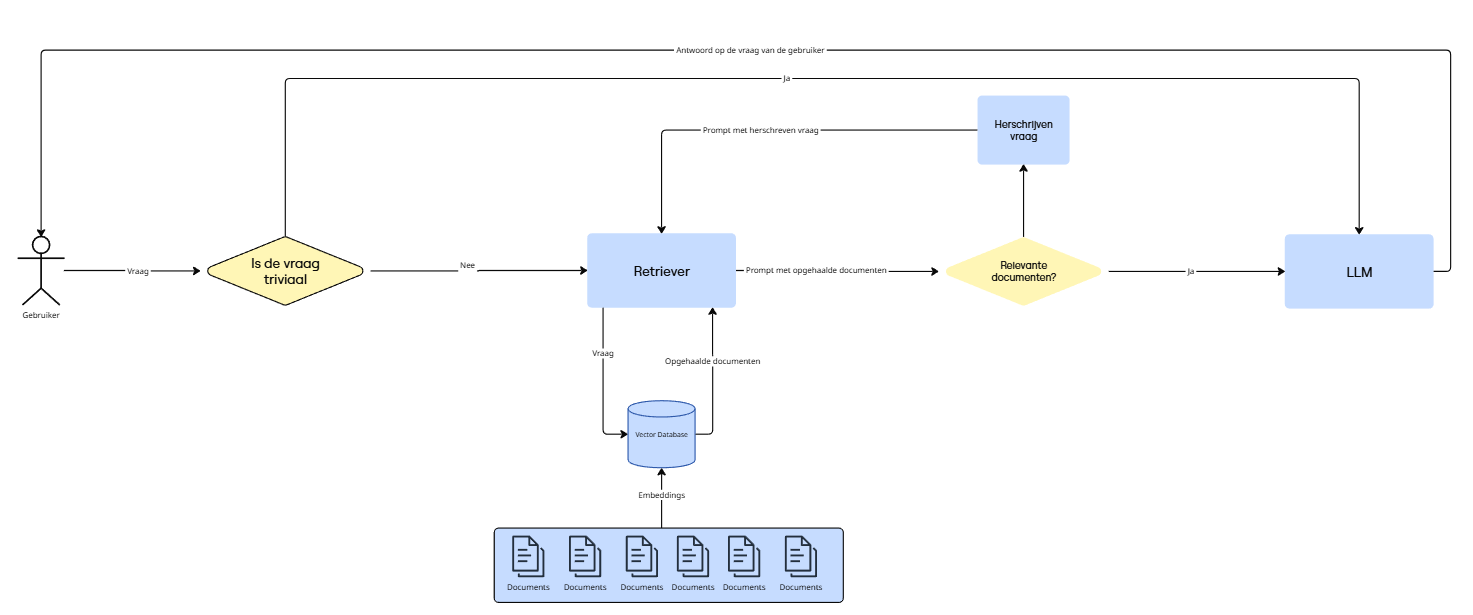
\includegraphics[width=1.0\linewidth]{flowchart_v2}
    \captionof{figure}{Overzicht van de structuur van de PoC met RAG-implementatie}
    \label{fig:PoC_RAG}
\end{center}

\section{Testscenario’s en Evaluatieopzet}

Voor de PoC werd een vergelijkende studie uitgevoerd met als doel de prestaties van verschillende modellen systematisch te evalueren. In dit kader werden de modellen Llama3.2, Llama3.1, Qwen2.5 en Qwen3 geselecteerd en onderworpen aan een reeks testscenario’s. Op basis van deze scenario’s kon worden vastgesteld welk model het meest adequaat presteerde.

In het eerste scenario werden tien vragen geformuleerd waarvan de antwoorden expliciet aanwezig waren in de beschikbare documentatie. De verwachting was dat het model op basis van de RAG-architectuur de relevante documenten correct zou ophalen en de gebruiker een accuraat antwoord zou verschaffen. De kwaliteit van de antwoorden werd geëvalueerd met behulp van het test framework \textit{Ragas}. 

Uit de resultaten bleek dat Qwen3 het beste model was, gevolgd door Llama3.2 en Llama3.1. Qwen2.5 presteerde het zwakst en slaagde er vaak niet in de gestelde vraag te beantwoorden. Hoewel Qwen3 gemiddeld de beste scores behaalde over de verschillende meetcriteria, was het verschil met Llama3.2 zeer klein en scoorde Llama3.2 consistenter. Daarom kan worden gesteld dat Llama3.2 in dit scenario de beste prestaties leverde. 

Het tweede scenario bestond uit vragen die niet in de documentatie terug te vinden waren. Dit scenario had als doel te onderzoeken in welke mate de verschillende modellen geneigd waren tot het genereren van hallucinaties en hoe zij met kennishiaten omgingen.  

Uit de resultaten bleek dat slechts één model hallucinaties vertoonde, namelijk Llama3.2. Dit model ging bij vier van de vijf vragen hallucineren, waardoor het in een reële situatie onbetrouwbaar is.

In het derde en laatste scenario werden triviale vragen gesteld. Gezien de architectuur van de PoC werd van de LLM verwacht dat het de database enkel zou raadplegen wanneer dit noodzakelijk was. Dit scenario bood de mogelijkheid om te beoordelen welk model het meest efficiënt en consistent inspeelde op het onderliggende ontwerpprincipe van de PoC.  

De resultaten tonen een duidelijk verschil tussen de Llama- en Qwen-modellen. Beide Llama-modellen raadpleegden de database ongeacht de vraag, terwijl de Qwen-modellen correct oordeelden over de trivialiteit van de vragen en dus rechtstreeks antwoord gaven. Hoewel dit geen invloed heeft op de inhoudelijke kwaliteit van de antwoorden, toont het wel aan dat de Qwen-modellen efficiënter omgaan met triviale vragen. Qua efficiëntie hebben de Qwen-modellen dus een duidelijk voordeel.

Op basis van de drie scenario’s kan worden geconcludeerd dat Qwen3 het best presterende model is. Het is het enige model dat in alle scenario’s degelijk scoorde en geen kritieke tekortkomingen vertoonde.


\section{Conclusies}

Op basis van de literatuurstudie en de scope van het onderzoek bleek dat RAG de meest geschikte methode is voor deze use case. De uitgewerkte PoC toont hoe RAG in de praktijk kan worden toegepast. Daarnaast kon een vergelijkende studie aantonen welk model het beste presteert, waarbij Qwen3 als meest geschikt naar voren kwam. Over het geheel genomen toont deze bachelorproef dat RAG een haalbare en veelbelovende aanpak is voor de ontwikkeling van een LLM-gebaseerde IT-support bot in de context van MyMinfin.


\section{Toekomstig onderzoek}
In toekomstig onderzoek kunnen de verschillende aspecten van het RAG-proces verder worden onderzocht. Voor deze PoC werden bepaalde onderdelen proefondervindelijk getest, maar dit betekent niet dat dit voor elke use case de beste oplossing is.

Daarnaast kan de impact van de modelgrootte bij RAG nader worden bekeken. In deze PoC werden verschillende modellen met elkaar vergeleken, maar het is ook interessant om te onderzoeken hoe verschillende groottes van hetzelfde model presteren.

Tot slot kunnen ook methoden zoals CAG of fine-tuning verder worden bestudeerd. In deze studie lag de focus op RAG, maar dit betekent niet dat CAG of fine-tuning geen waardevolle opties zijn voor andere toepassingen. Het verdient dus zeker de moeite om deze benaderingen verder te onderzoeken.

\end{multicols}
\end{document}